\documentclass{article}
\usepackage[letterpaper,top=1cm,bottom=2cm,left=1cm,right=1cm,marginparwidth=1.75cm]{geometry}
\usepackage{bm}
\usepackage{amsmath}
\usepackage{graphicx}
\graphicspath{ {./} }

\title{ESC210 Final}
\author{Jake Sigman}
\date{}

\begin{document}


\section*{Definitions}

\begin{description}
    \item[Alloy] A mixture of metal with other metals or non-metals.
    \item[Phase] A region of material that has homogenous properties and composition.
    \item[Components] The chemical elements which make up alloys.
    \item[Microstructure] The distribution of the phases in a solid alloy.
\end{description}

\section*{Reading Phase Diagrams}

\begin{description}
    \item[Temperature of first liquid phase] \(183^\circ\)C
    \item[Composition of liquid phase] 61.9 wt\% Sn
    \item[Temperature of complete melting] \(250^\circ\)C
    \item[Composition of last solid prior to melting] 15 wt\% Sn
    \item[Mass of lead in alloy] \(8\,\textnormal{kg} * 20\%=\textit{1.6 kg}\)
\end{description}
\subsection*{How much more lead may be dissolved in \(\alpha\)-phase}
Let \(x\) be the amount of Pb added (kg).
\[\frac{1.6 \textnormal{ kg}+x}{8 \textnormal{ kg}+x}=30 \textnormal{ wt\%}\]
\[1.6 \textnormal{ kg}+x=0.3*8\textnormal{ kg}+0.3x\]
\[0.7x=0.8\hspace{7 mm}x=\textit{1.14 kg}\]

\section*{The Lever Rule}
\subsection*{Determining the Composition of the \(\beta\)-phase}
\[\frac{40 \textnormal{ wt\% B}-13 \textnormal{ wt\% B}}{x \textnormal{ wt\% B}-13 \textnormal{ wt\% B}}=0.5\]
\[x=\textit{67 wt\% B}=\textit{33 wt\% A}\]
\subsection*{Determining the mass fractions of the \(\alpha\) and \(\beta\) phases}
\[\frac{90 \textnormal{ wt\% Sn}-18.3 \textnormal{ wt\% Sn}}{97.8 \textnormal{ wt\% Sn}-18.3 \textnormal{ wt\% Sn}}=\textit{0.9 } \mathit{\beta}=\textit{0.1 } \mathit{\alpha}\]
\subsection*{Determining the mass fractions of the primary \(\beta\) and eutectic microconstituents}
\[\frac{90 \textnormal{ wt\% Sn}-61.9 \textnormal{ wt\% Sn}}{97.8 \textnormal{ wt\% Sn}-61.9 \textnormal{ wt\% Sn}}=\textit{0.78 Pre-Eutectic } \mathit{\beta}=\textit{0.22 Eutectic}\]
\subsection*{Determining the mass fraction of eutectic \(\beta\)}
\[0.9 \textnormal{ Total } \beta-0.78 \textnormal{ Pre-Eutectic } \beta=\textit{0.12 Eutectic } \mathit{\beta}\]
\subsection*{Determining the composition of an alloy}
\[\frac{C_0-64 \textnormal{ wt\%}}{x-64 \textnormal{ wt\%}}=0.367\hspace{10 mm}\frac{C_0-12 \textnormal{ wt\%}}{x-12 \textnormal{ wt\%}}=0.768\]

$$
\left[\begin{matrix}
\frac{1}{\textnormal{Primary } \beta} & -1\\\\
\frac{1}{\textnormal{Total } \beta} & -1
\end{matrix}
\left|\begin{matrix}
-\textnormal{wt\%}_\textnormal{Eutectic}+\frac{\textnormal{wt\%}_\textnormal{Eutectic}}{\textnormal{Primary   }\beta}\\\\
-\textnormal{wt\%}_\textnormal{Eutectic}+\frac{\textnormal{wt\%}_\textnormal{Eutectic}}{\textnormal{Total   }\beta}
\end{matrix}
\right.
\right]=
\left[\begin{matrix}
\frac{1}{0.367} & -1\\\\
\frac{1}{0.768} & -1
\end{matrix}
\left|\begin{matrix}
-64\textnormal{ wt\%}+\frac{64 \textnormal{ wt\%}}{0.367}\\\\
-12\textnormal{ wt\%}+\frac{12 \textnormal{ wt\%}}{0.768}
\end{matrix}
\right.
\right]=
\left[\begin{matrix}
C_0 & 0\\\\
0 & x
\end{matrix}
\left|\begin{matrix}
75.04 \textnormal{ wt\% B}\\\\
94.08 \textnormal{ wt\%}
\end{matrix}
\right.
\right]
$$
\[C_0=\mathit{75.04 \textit{ wt\% B}}=\textit{24.96 wt\% A}\]
\section*{Example Phase Diagram}
\begin{center}
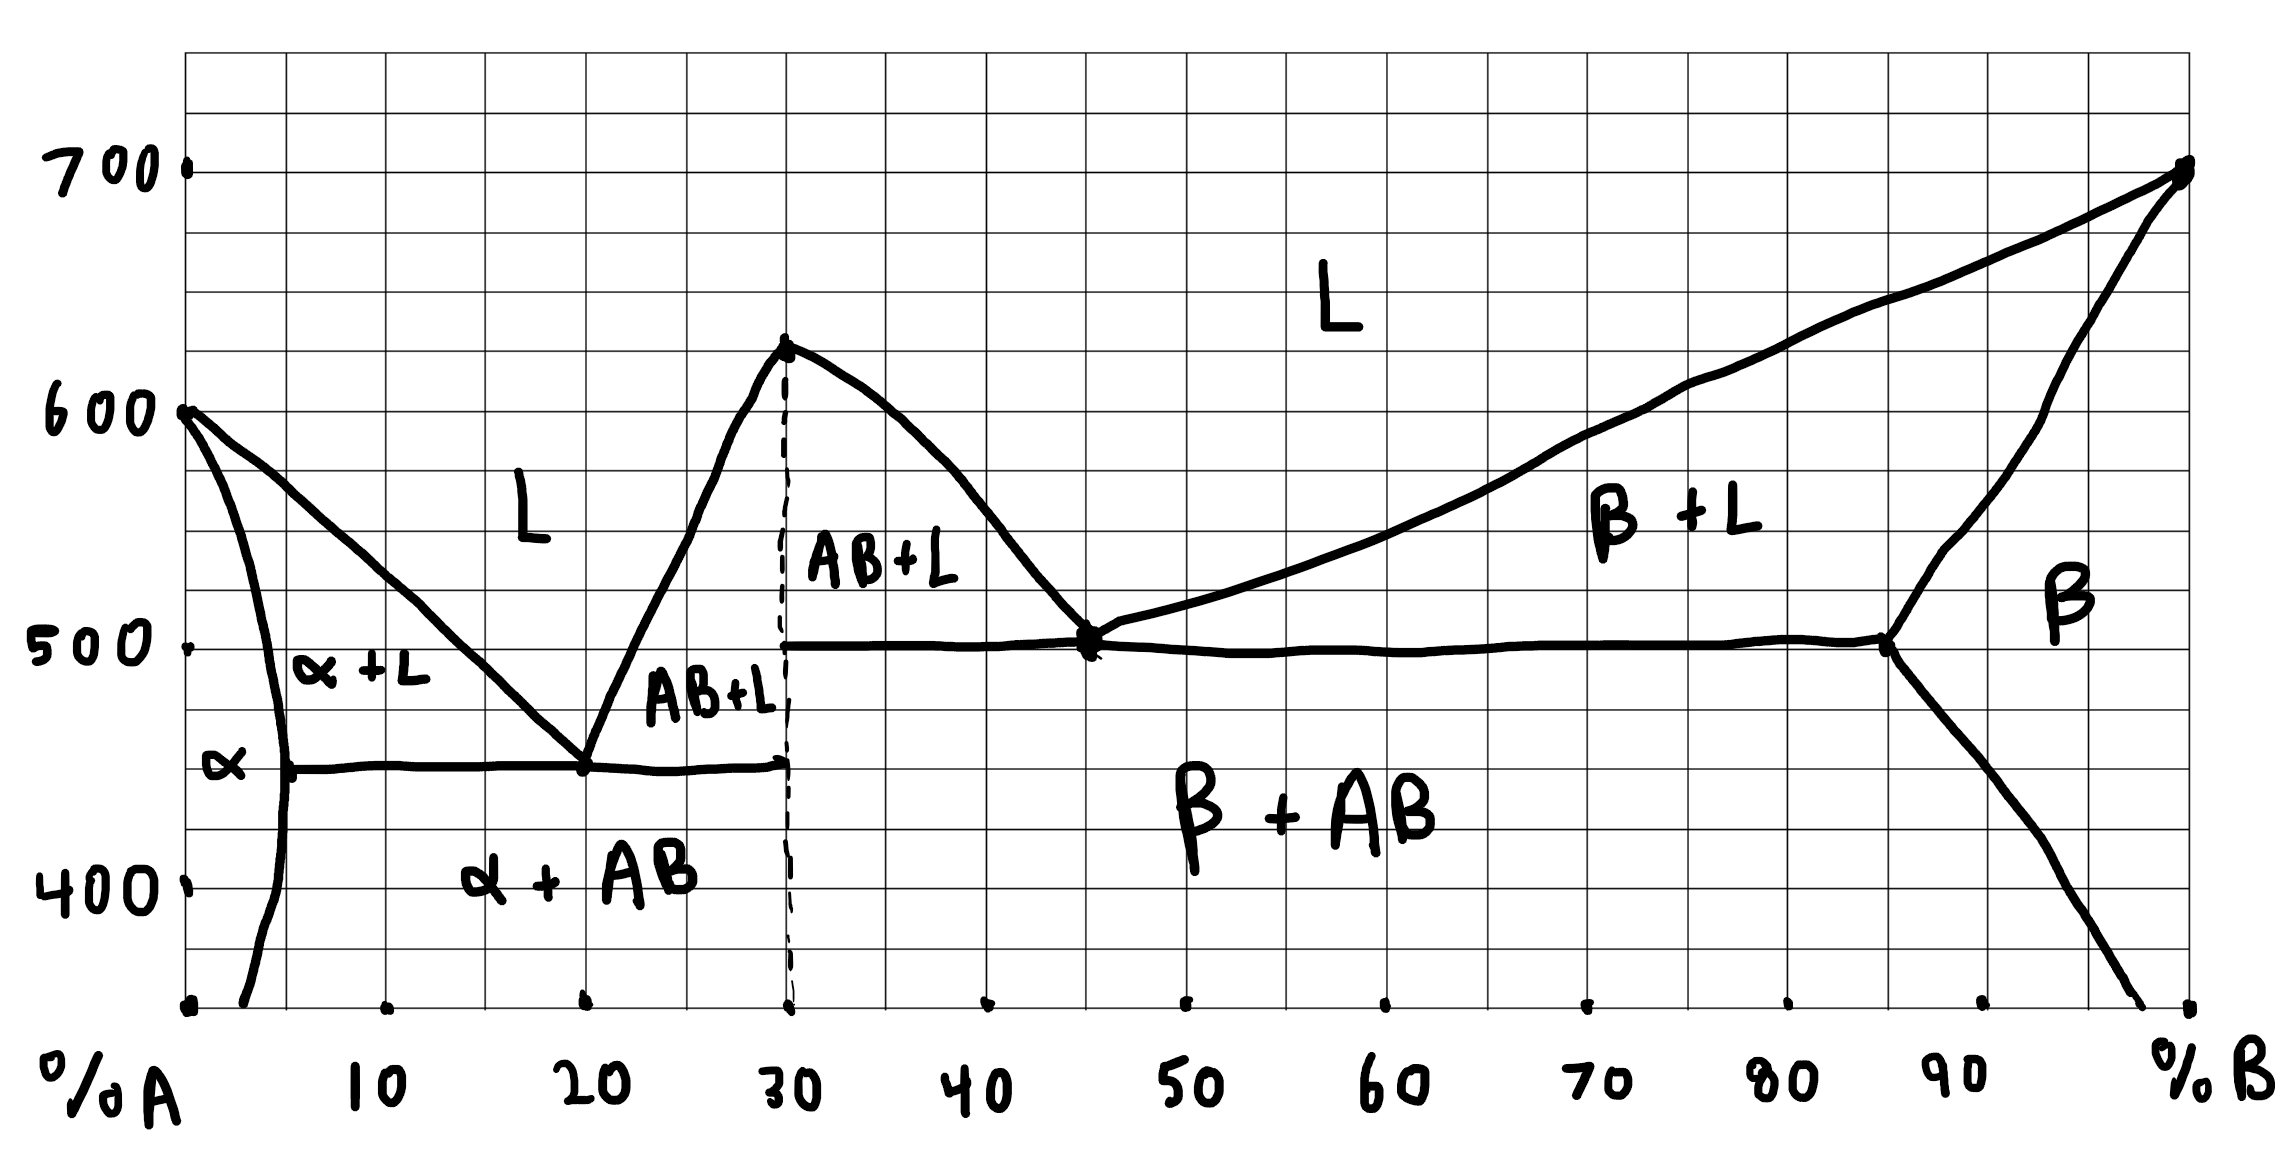
\includegraphics[scale=0.33]{Question 7.png}
\end{center}

\section*{Calculating Mass and Weight Percent}
\[\textnormal{Total Gold}=3*50\textnormal{ g}*40\textnormal{ wt\%}+7*100\textnormal{ g}*60\textnormal{ wt\%}+9*30\textnormal{ g}*50\textnormal{ wt\%}=615 \textnormal{ g}\]
\[\textnormal{Total Silver}=3*50\textnormal{ g}*60\textnormal{ wt\%}+7*100\textnormal{ g}*40\textnormal{ wt\%}+9*30\textnormal{ g}*50\textnormal{ wt\%}=505 \textnormal{ g}\]
\[\textnormal{Total Weight}=\textnormal{Total Gold}+\textnormal{Total Silver}=615 \textnormal{ g}+505 \textnormal{ g}=1120 \textnormal{ g}\]
\[\textnormal{wt\% Gold}=\frac{\textnormal{Total Gold}}{\textnormal{Total Weight}}*100=\frac{615 \textnormal{ g}}{1120 \textbf{ g}}*100=55\textnormal{ wt\%}\]
Since Ericth Limaneth isolated the solid part, a line must be drawn to the \(\alpha\) phase to determine the weight percent gold of the solid part. Once the line is drawn, the weight percent is determined to be \textit{65 wt\%}. Then, the mass fraction is calculated using the lever rule.
\[W_\alpha=\frac{55 \textnormal{ wt\%}-50 \textnormal{ wt\%}}{65 \textnormal{ wt\%}-50 \textnormal{ wt\%}}=\frac{1}{3}\]
Multiple the total weight calculated by the mass fraction to obtain the weight of the new ring.
\[W_\alpha*\textnormal{Total Weight}=\frac{1}{3}*1120\textnormal{ g}=\mathit{373.33} \textit{ g}\]
\section*{More on Phases}
The proeutectoid phase is called \textit{Ferrite} and the eutectoid microstructure for the iron-carbon system is called \textit{Pearlite}.\\
\[\frac{0.45 \textnormal{ wt\%}-0.022 \textnormal{ wt\%}}{0.76 \textnormal{ wt\%}-0.022 \textnormal{ wt\%}}*6\textnormal{ kg}=\textit{3.48 kg Eutectoid}\]
\[\textnormal{Proeutectoid}=6\textnormal{ kg}-3.48\textnormal{ kg}=\mathit{2.52}\textit{ kg Proeutectoid}\]
\begin{center}
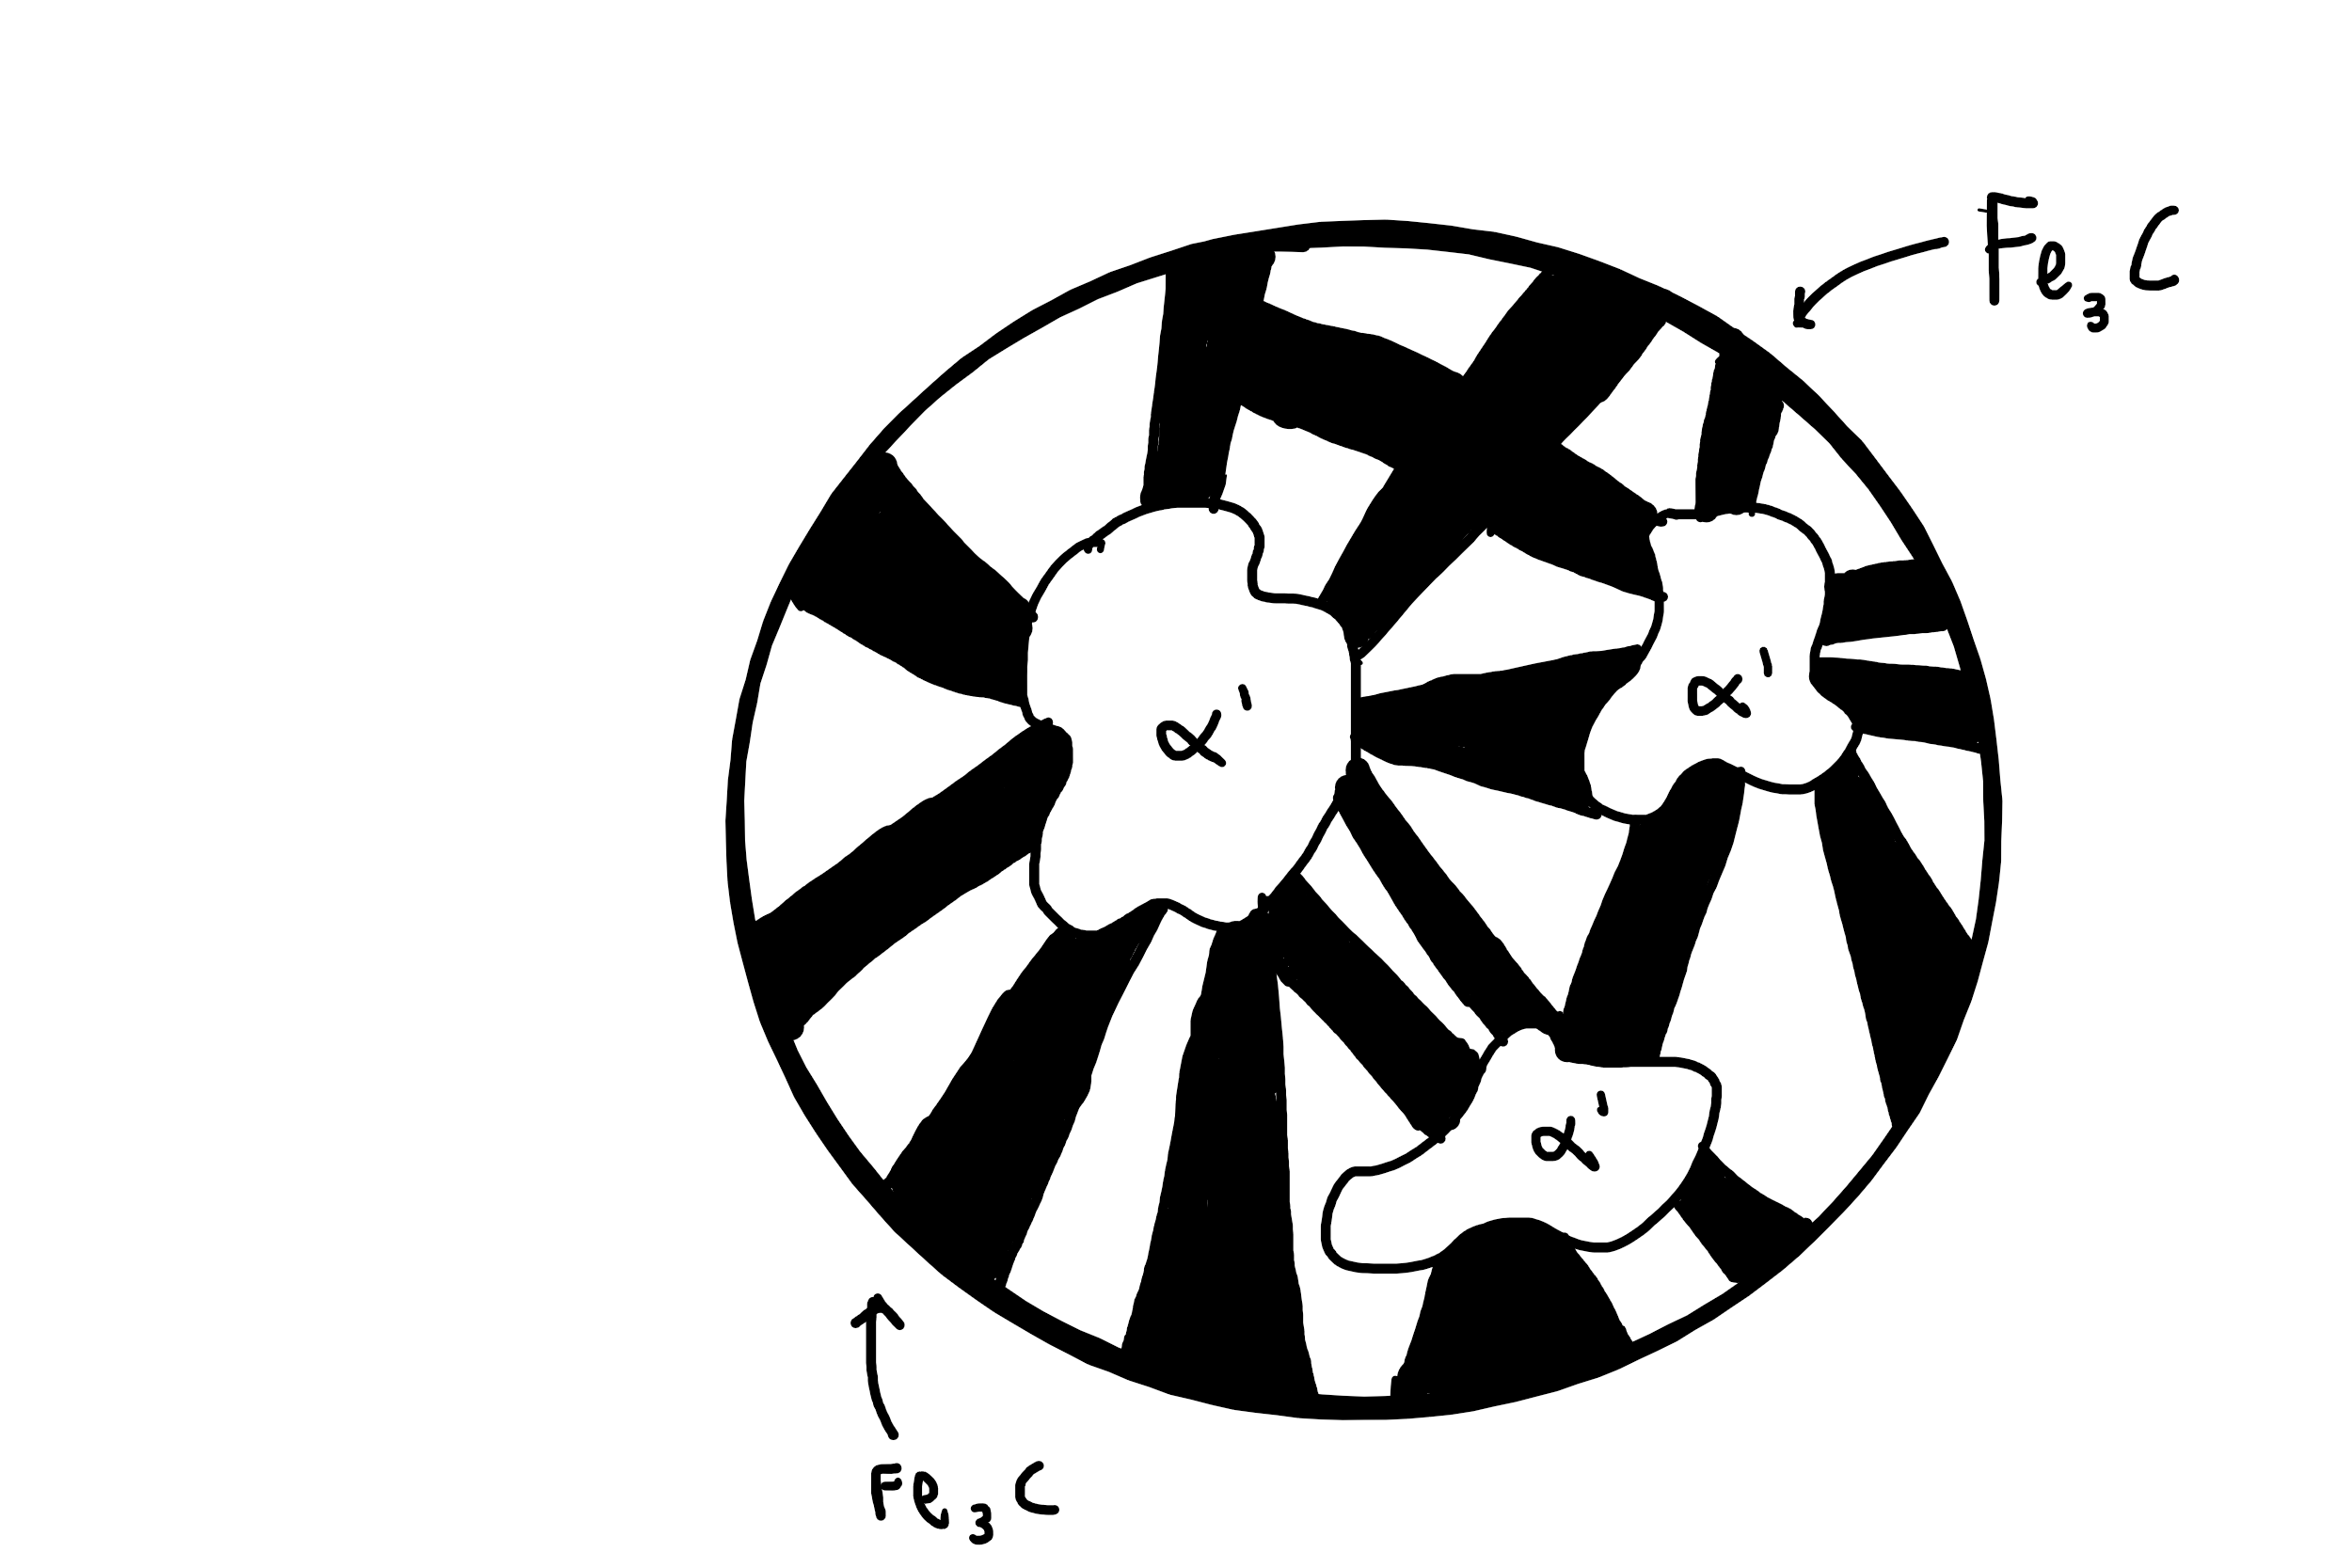
\includegraphics[scale=0.12]{Question 13.png}
\end{center}
\end{document}
